\setcounter{chapter}{9}
\chapter{Mehrdimensionale Differenzialrechnung}

Wir wollen in diesem Kapitel den Begriff des Grenzwertes und der Ableitung für Funktionen von $\R^n$ in $\R^m$ definieren. Wie auch bei der eindimensionalen Ableitung müssen wir zuerst den Begriff der (punktierten) Umgebung und den des Häufungspunktes definieren:
\section{Begriffe}
\begin{definition}{punktierte Umgebung}{}
Sei $X$ ein metrischer Raum und $x_0\in X$. Die \textbf{punktierte Umgebung} von $x$ ist
$$\Dot{D}_\varepsilon(x_0) = B_\varepsilon(x_0) \setminus \{x_0\} = \set{x\in X}{0 < d(x, x_0) < \varepsilon}$$
\end{definition}
\begin{definition}{Häufungspunkt}{}
Sei $D \subseteq X$ eine Teilmenge des metrischen Raums $X$. $x_0 \in X$ heisst \textbf{Häufungspunkt} von $D$, falls für alle $\varepsilon > 0$ der Schnitt der punktierten Umgebung $\Dot{B}_\varepsilon(x_0)$ mit $D$ nicht-leer ist:
$$x_0 \text{ Häufungspunkt von } D \iff \forall \varepsilon > 0: \Dot{B}_\varepsilon(x_0) \cap D \neq \emptyset$$
\end{definition}
\begin{definition}{Grenzwert einer Funktion}{}
Sei $f:D \to Y$ mit $D \subseteq X$ ein Teilraum und $x_0$ ein Häufungspunkt von $D$, dann bedeutet
$$\lim_{y\to x_0} f(y) = a \iff \forall \varepsilon > 0 \ \exists \delta>0: y \in D \cap \Dot{B}_\delta(x_0) \implies f(y) \in B_\varepsilon(a)$$
Äquivalent dazu: Für alle Folgen $(x_n)_{n \in \N} \subseteq D$ mit $\lim_{n \to \infty}x_n = x_0$ gilt:
$$\lim_{n \to \infty} f(x_n) = a$$
\end{definition}
\begin{korollar}{Stetigkeit}{}
Eine Funktion $f: D \to Y$ mit $D\subseteq X$ ein Teilraum ist genau dann stetig, wenn für alle Häufungspunkte $x_0 \in D$ gilt:
$$\lim_{x \to x_0} f(x) = f(x_0)$$
\end{korollar}
\begin{proof}
Dies folgt direkt aus der Definition der Stetigkeit \ref{cha_stetigkeit_metr} und der obigen Definition des Grenzwertes.
\end{proof}
Für eine ausführlichere Erklärung und Motivation dieser Begriffe siehe Abschnitt \ref{cha_grundlagen_diffrechnung}.

\section{Die Ableitung}
Wir erinnern uns nochmal an die Eigenschaften der Ableitung in $\R$: Sei $D \subseteq \R$ offen, dann ist $f: D \to \R$ bei $x_0 \in D$ differenzierbar, wenn es eine lineare Funktion $f'(x_0): D \to \R, h \mapsto f'(x_0) \cdot h$ gibt, sodass gilt:
$$f(x_0 + h) = f(x_0) + f'(x_0)h + o(\abs{h})$$
Daraus können wir die (affin)lineare Approximation von $f$ durch $f(x_0) + f'(x_0)(x-x_0)$ herleiten, welche $f$ bei Punkten nahe an $x_0$ beliebig genau approximieren kann.
Dadurch ist $f'$ eindeutig bestimmt und es gilt
$$\frac{o(\abs{h})}{\abs{h}} = \abs{\frac{f(x_0+h)- f(x_0)}{h} - f'(x_0)} \longrightarrow 0 \quad (h \to 0)$$
Siehe Abschnitt \ref{cha_landau_notation} für Details zur Landau-Variante der Ableitung.

Wir wollen nun einen allgemeinen, koordinatenunabhängigen Begriff der Ableitung definieren (also ohne Basis):
\begin{definition}{Ableitung}{}
Seien $V,W$ endlichdimensionale normierte Vektorräume über $\R$ und sei $U \subseteq V$ ein offener Teilraum. Die Abbildung $f: U \to W$ nennen wir \textbf{differenzierbar} bei $x_0 \in U$, wenn es eine eindeutige lineare Abbildung $f'(x_0): V \to W, h \mapsto f'(x_0)\cdot h$ gibt, sodass für $x_0, x_0+h \in U$ gilt
\begin{align}\label{eq_totales_differential}
    f(x_0+h) = f(x_0) + f'(x_0) h + o(\norm{h}) \longrightarrow 0 \quad (h \to 0)
\end{align}
wobei $o(\norm{h}): \R \to W$ hierbei eine Abbildung ist, die $\lim_{h \to 0} \frac{\norm{o(\norm{h}_V)}_W}{\norm{h}_V} = 0$ erfüllt.

Dies ist die (totale) \textbf{Ableitung}/das Differenzial/Tangentialabbildung und wir schreiben $D_{x_0}f$ oder $Df(x_0), df(x_0),f'(x_0),...$. Zudem heisst $f: U \to W$ \textbf{differenzierbar}, wenn $f$ bei allen $x_0 \in U$ differenzierbar ist.
\end{definition}
Alternativ könnte man auch eine Folge $(h_{i})_{i \in \N}$ in $\R^n\setminus\{0\}$ mit $x_0 + h_i \in U$ für alle Folgenglieder und $\lim_{i \to \infty} h_i = 0$ betrachten, dann gilt für die Ableitung:
$$\lim_{i \to \infty}\frac{\norm{f(x_0 + h_i) - f(x_0)  - f'(x_0) h_i}_W}{\norm{h_i}_V} = 0$$
\begin{remark}
Beachte, dass $f'$ eine Abbildung von $U \to \text{Hom}(V, W)$ mit $x_0 \mapsto f'(x_0) \in \text{Hom}(V, W)$ ist, also ist $f'(x_0)$ eine lineare Abbildung von $V \to W$, welches ein Element $h \in V$ nach $W$ abbildet. Wir werden $f(x_0)$ als Matrix darstellen, welche einen Vektor $h \in U$ aufnimmt und einen anderen Vektor $f(x_0)(h) \in W$ zurückgibt. Daher können wir den Definitionsbereich von $f'(x_0)$ auch ganz $V$ verwenden, da wie in $\R$ die Tangente über ganz $\R$ definiert ist.
\end{remark}

\subsection{Richtungsableitung}
Schränken wir die Ableitungsrichtung durch einen Vektor ein, so erhalten wir den Begriff der \textbf{Richtungsableitung}:
\begin{definition}{Richtungsableitung}{}
Sei $U \subseteq V$ und $f: U \to W$ differenzierbar in $x_0$, dann ist die Ableitung von $f$ entlang eines Vektors $v \in V$ bei $x_0 \in U$ die \textbf{Richtungsableitung} in Richtung $v$
$$\partial_v f(x_0) = \lim_{t \to 0} \frac{f(x_0 + tv) - f(x_0)}{t} = \diff{}t f(x_0+ tv) \Big\vert_{t=0}$$
\end{definition}
\begin{remark}
Beachte, dass auch hier die Richtungsableitung auf für Vektoren $v \notin U$ definiert ist. 
\end{remark}
\begin{lemma}{Richtungsableitung in beliebige Richtungen}{}
Falls $f$ bei $x_0 \in U$ differenzierbar ist, dann existiert auch die Richtungsableitung
$$\partial_v f(x_0) = f'(x_0)v$$
für beliebige $v \in V$. Insbesondere ist die lineare Abbildung $f'(x_0)$ eindeutig durch (\ref{eq_totales_differential}) bestimmt.
\end{lemma}
Die Ableitungsmatrix $f'(x_0)$ enthält also sozusagen alle Informationen für beliebige Richtungsableitungen.
\begin{proof}
Sei $v \neq 0 \in V$ und $h = tv$ mit $t \in \R$, dann gilt mit der Definition der (totalen) Ableitung:
$$f(x_0 + tv) = f(x_0) + f'(x_0)tv + \underbrace{o(\norm{tv})}_{=: R(t)} = f(x_0) + tf'(x_0)v + R(t)$$
Es folgt mit $\lim_{t \to 0} \frac{\norm{R(t)}}{tv} = 0$
\begin{align*}
    \lim_{t\to 0} \frac{\norm{f(x_0+ tv) -f(x_0) -f'(x_0)tv}}{\abs{t}\norm{v}} &= 0\\ 
    \lim_{t\to 0} \frac{1}{\norm{v}}\norm{\frac{f(x_0+ tv) -f(x_0)}{t}-f'(x_0)v} &= 0
\end{align*}
Also erhalten wir wie behauptet
$$\underbrace{\lim_{t \to 0} \frac{f(x_0 + tv) - f(x_0)}{t}}_{\partial_v f(x_0)}= f'(x_0) v$$
Für $v=0$ sind beide Seiten $=0$, da das eine Eigenschaft von linearen Abbildungen ist. Die Eindeutigkeit von $f'(x_0)$ folgt, weil wir für einen beliebigen Vektor $v$ zeigen konnten, dass die lineare Abbildung $f'(x_0)v = \partial_v f(x_0)$ eindeutig ist (siehe Definition von $\partial_v f(x_0)$, diese ist nicht abhängig von $f'(x_0)$).
\end{proof}

\begin{example}
Sei $f: \R^2 \to \R$ eine Abbildung mit $(x,y) \mapsto xy + \cos(y)$, dann erhalten wir für die Richtungsableitung in Richtung $v = \binom{v_1}{v_2}$:
\begin{align*}
    \partial_vf(x_0,y_0) &= \diff{}{t} f\binom{x_0 + tv_1}{y_0 + tv_2}\Big\vert_{t=0}\\
    &= \diff{}{t} (x_0 + tv_1)(y_0 + tv_2) + \cos(y_0 + tv_2) \Big\vert_{t=0}\\
    &= v_1 y_0 + x_0v_2 - v_2 \sin (y_0)
\end{align*}
\end{example}

\subsection{Partielle Ableitung}
Wir möchten nun den Begriff der Ableitung im Bezug auf eine Basis von $V = \R^n$ resp. $W = \R^m$ betrachten.

\begin{lemma}{}{}
Sei $U \subseteq \R^n$ eine offene Menge und $f: U \to \R^m$ eine differenzierbare Funktion mit $f(x) = (f_1(x), ..., f_m(x))^T$ und $v\in \R^n$, dann gilt
$$\partial_vf(x) = \mat{\partial_vf_1(x)\\ \vdots \\ \partial_v f_m(x)}$$
\end{lemma}
\begin{proof} Wir setzten in die Definition ein und erhalten direkt die Behauptung:
\begin{align*}
    \partial_vf(x) &= \lim_{t\to 0} \frac{f(x+tv) -f(x)}{t}\\
    &= \mat{\lim_{t\to 0} \frac{f_1(x+tv) -f_1(x)}{t}\\ \vdots \\ \lim_{t\to 0} \frac{f_m(x+tv) -f_m(x)}{t}}
\end{align*}
\end{proof}
Da $f'$ eine lineare Abbildung i.e. Homomorphismus $V \to W$ ist, brauchen wir für die explizite Konstruktion von $f'(x)$ nur zu wissen, wohin die Basisvektoren von $U = \R^n$ abgebildet werden, und können diese in die Spalten einer Matrix eintragen. Die Richtungsableitung von Basisvektoren nennen wir die \textbf{partielle Ableitung}:
\begin{definition}{partielle Ableitung}{}
Für Einheitsvektoren $v = e_i$ einer Basis $(e_1, ..., e_n)$ von $\R^n$ definieren wir die \textbf{partielle Ableitung}
$$\diffp{f}{x_i}(x) := \partial_{e_i}f(x) = \lim_{t\to 0}\frac{f(x_1, ..., x_{i}+t, ..., x_n) - f(x_1, ..., x_{i}, ..., x_n)}{t}$$
\end{definition}
Also ist $\diffp{f}{x_i}(x) \in W$ die Ableitung von $f$ nach der Variablen $x_i$ im Punkt $x$ ist, wobei alle anderen $x_j, j\neq i$ festgehalten werden.

\subsection{Jacobi-Matrix}
Tragen wir nun die partiellen Ableitungen $f'(x)e_i = \diffp{f}{x_i}(x)$ der Basisvektoren der Standardbasis in die Spalten der Matrix von $f'(x)$ ein, so konnten wir $f'(x)$ explizit berechnen und wir erhalten die $m \times n$ \textbf{Jacobi-Matrix}: 

\begin{definition}{Jacobi-Matrix}{}
\begin{align*}
    D_xf = \mat{\vert& & \vert \\\diffp{f}{x_1}(x) & \cdots & \diffp{f}{x_n}(x) \\ \vert & & \vert } = \mat{\diffp{f_1}{x_1}(x) & \cdots & \diffp{f_1}{x_n}(x)\\
    \vdots & \ddots & \vdots \\
    \diffp{f_m}{x_1}(x) & \cdots & \diffp{f_m}{x_n}(x) } =
    \mat{(\nabla f_1)^T\vert_{x}  \\ \vdots  \\  (\nabla f_m)^T\vert_{x} } \in M_{m \times n}
\end{align*}
\end{definition}
Es gilt also
$$f'(x) \cdot v = \partial_v f(x) = \mat{\partial_vf_1(x)\\ \vdots \\ \partial_v f_m(x)} = \mat{v_1\diffp{f_1}{x_1}(x) & \cdots & v_n\diffp{f_1}{x_n}(x)\\
    \vdots & \ddots & \vdots \\
    v_1\diffp{f_m}{x_1}(x) & \cdots & v_n\diffp{f_m}{x_n}(x) } = D_xf \cdot v$$
Beachte die Verwendung des Subskripts der Richtungsableitung resp. der Jacobi-Matrix: Ersteres verwendet es als Ableitungsrichtung, letzteres als Auswertungsstelle.

\begin{example}
Sei $V = \R^2$ und $W= \R^1$, dann ist der Graph einer Funktion $f: \R^2 \to \R$ eine Fläche im $R^3$, hier in blau. In einem Punkt $P = (x,y, f(x,y))$ bildet $z = f(x_0, y_0) + D_{x_0, y_0}f\cdot \binom{x-x_0}{y-y_0}$ eine Tantentialebene in rot an den Graphen:
\begin{center}
    \centering
    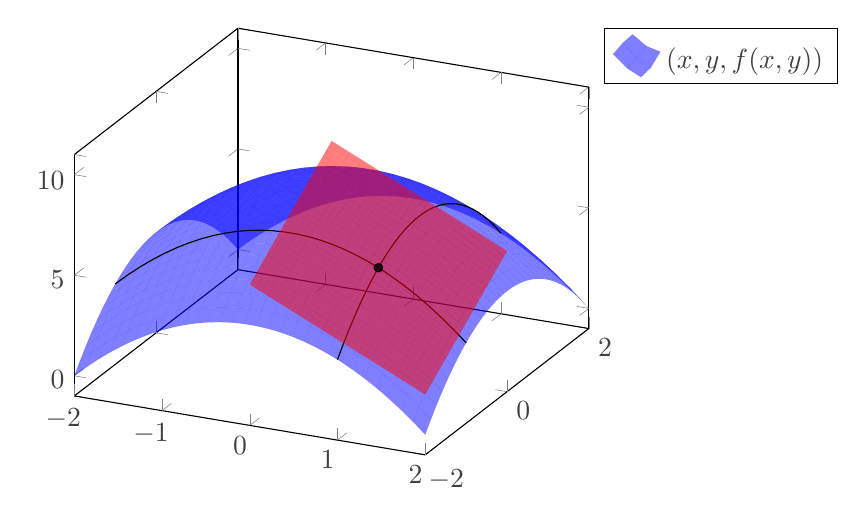
\begin{tikzpicture}
    \begin{axis}[%colormap/viridis,
    height=7cm,
    surf, fill opacity=0.75,
    grid style=dashed,
    legend pos=outer north east
    ]
    \addplot3[surf,domain=-2:2,samples=30, opacity=0.01, fill opacity = 0.5, blue, shader=flat] {8 - x*x - y*y};
    \addplot3[mark=*, mark size=1.5] coordinates{(1,-1,6)}; 
    \addplot3[domain=-2:2, samples = 30, samples y=0] ({x}, {-1}, {7 - x*x});
    \addplot3[domain=-2:2, samples = 30, samples y=0] ({1}, {x}, {7 - x*x});
    \addplot3[surf,domain=0:2,samples=30, opacity=0.01, fill opacity = 0.5, red, shader=flat] ({x}, {-y}, {10 - 2*x - 2*y});
    \addlegendentry{$(x,y,f(x,y))$}
    \end{axis}
    \end{tikzpicture}
\end{center}
\end{example}

Wir können für ein stetiges $f$ die Konvergenzbedingung der Differenzierbarkeit auch so formulieren:
$$\mat{f_1(x+h)  \\ \vdots  \\  f_m(x+h) } =
\mat{f_1(x)  \\ \vdots  \\  f_m(x) } +
(D_xf)\mat{h_1  \\ \vdots  \\  h_n} + o(\norm{h}_V)  \longrightarrow 0 \quad (h \to 0)$$
Ganz wichtig ist jetzt aber, dass die umgekehrte Implikation im Allgemeinen \textbf{nicht} gilt! Falls also eine Funktion obige Konvergenz aufweist, heisst das nicht, dass sie auch differenzierbar ist (Das gilt auch, wenn alle Richtungsableitungen möglichen definiert sind):
\begin{example}
Sei $f: \R^2 \to \R$ mit
$$f(x_1,x_2) = \begin{cases} \frac{x_1x_2}{\sqrt{x_1^2+ x_2^2}} & ,(x_1, x_2) \neq (0,0) \\ 0 & , (x_1, x_2) = (0,0)\end{cases}$$
Wir erkennen, dass $\diffp{f}{x}, \diffp{f}{y}$ für alle Punkte $(x,y)$ ausser $(0,0)$ existieren. Wir berechnnen nun  $\diffp{f}{x}(0,0)$:
$$\diffp{f}{x} = \lim_{t \to 0} \frac{f(t,0) - f(0,0)}{t} =  \lim_{t \to 0} \frac{0 - 0}{t} = 0$$
Wir erhalten $0$, da $f(t,0) = 0$ für jedes $t$ gilt. Analog erhalten wir $\diffp{f}{y}(0,0) = 0$. Somit existieren beide partiellen Ableitungen für jedes $x \in \R^2$.

Betrachten wir nun aber die Richtungsableitung entlang von z.B. $v = \binom{1}{1}$, so sehen wir, dass $\partial_vf$ bei $0$ nicht definiert ist:
$$f(0+t, 0+t) = \frac{t^2}{\sqrt{2t^2}} = \frac{\abs{t}}{\sqrt{2}}$$
Es folgt, dass $f$ bei $(0,0)$ nicht differenzierbar ist:
$$\lim_{t \searrow 0}\frac{f(t,t)-f(0,0)}{t} = \lim_{t \searrow 0} \frac{\abs{t}}{\sqrt{2}t} = \frac{1}{\sqrt{2}} \neq -\frac{1}{\sqrt{2}} = \lim_{t \nearrow 0} \frac{\abs{t}}{\sqrt{2}t}$$
\end{example}

Wir können jedoch folgenden Satz formulieren, mit welchem wir auf die Differenzierbarkeit von $f$ schliessen können:
\begin{satz}{Differenzierbarkeit und partielle Ableitungen}{}
Sei $f: U \to \R^m$ mit $U \subseteq \R^n$ eine Abbildung. Falls alle partiellen Ableitungen $\diffp{f_i}{x_j}$ existieren und falls für alle $i\leq m, j \leq n$ die Abbildungen
$$x \mapsto \diffp{f_i}{x_j}(x)$$
stetig sind, dann ist $f$ differenzierbar.
\end{satz}
\begin{definition}{stetige Differenzierbarkeit}{}
Sei $U \subseteq\R^n$ offen und $f:U \to \R^m$ eine Funktion, dann heisst $f$ \textbf{stetig differenzierbar}, wenn alle partiellen Ableitungen $\diffp{f_i}{x_j}$ existieren und stetig sind auf $U$.

Also ist die vektorwertige Abbildung, die einem Punkt die Ableitungsmatrix zuordnet, stetig:
$$x \mapsto D_xf = \bk{\diffp{f_i}{x_j}}_{ij} \in M_{m \times n}(\R)$$
\end{definition}
Falls also $f$ \textbf{stetig differenzierbar} ist, so lässt sich die Ableitung finden.
\begin{remark}
Wir können die Stetigkeit mit einer beliebigen Norm von $\R^n$ zeigen, da sie alle dieselbe Topologie induzieren (Satz \ref{satz:equiv_real_norms}), jedoch ist die \textbf{Operatornorm} $\Nrm_{op}$ natürlich/kanonisch für $\text{Hom}(\R^n, \R^m)$:
$$\norm{A}_{op} = \sup \set{\norm{Ax}}{x \in \R^n, \norm{x} \leq 1}$$
Die Operatornorm erfüllt $\norm{Ax} \leq \norm{x} \norm{A}_{op}$ und $\norm{AB}_{op} \leq \norm{A}_{op} \norm{B}_{op}$
\end{remark}

\subsection{Spezielle Jacobi-Matrizen}
Wir wollen noch einige spezielle Jacobi-Matrizen betrachten:
\begin{itemize}
    \item Mit $n=1$ betrachten wir Wege in $\R^m$ von der Form $t\mapsto \gamma(t) = \bk{\gamma_1(t), \cdots, \gamma_m(t)}^T \in \R^m$. $D_t\gamma$ ist somit einen $m \times 1$ Spaltenvektor:
    $$D_t\gamma = \mat{
    \Dot{\gamma}_1(t)\\ \vdots \\ \Dot{\gamma}_m(t)
    }$$
    wobei wir mit $\Dot{\cdot} = \diff{}{t}$ den Geschwindigkeitsvektor bezeichnen. Es gilt also mit $h \in \R$:
    $$\gamma(t+h) = \gamma(t) + \Dot{\gamma}(t)h + o(\abs{h})$$
    \item Mit $m = 1$ betrachten wir ein Skalarfeld $x\in \R^n \mapsto f(x) = f(x_1,...,x_n) \in \R$. Also ist $D_xf$ gegeben durch einen $1\times n$ Zeilenvektor:
    $$D_xf = \mat{ \diffp{f}{x_1}(x) & \hdots & \diffp{f}{x_n}(x)  }$$
    Wir erhalten also
    $$f(x+h) = f(x) + (D_xf)h + o(\norm{h}) = f(x) + \sum_{i=1}^n \diffp{f}{x_i}(x)h_i + o(\norm{h})$$
    Dabei spricht man oft vom \textbf{Gradient} $\nabla f(x)$, welcher in der Literatur als Spaltenvektor definiert ist:
    $$\nabla f(x) = \mat{ \diffp{f}{x_1}(x) \\ \vdots \\ \diffp{f}{x_n}(x)  }$$
    wobei dann mit $\nabla f(x) \cdot h$ auch das Standardskalarprodukt auf $\R^n$ gemeint ist.
    
    Wenn wir die Richtungsableitung $\partial_vf$ eines normierten Vektors $v \in \R^m, \norm{v} = 1$ betrachten, können wir mit der Cauchy-Schwarz Ungleichung
    $$a\cdot b = \norm{a}\norm{b} \cos \theta$$
    wobei $\theta = \angle(a,b)$ der Winkel zwischen den Vektoren ist, folgende Aussage herleiten: Sei $a = v$ und $b = \partial_vf = \nabla f\cdot v$:
    $$\partial_vf(x) = \norm{\nabla f(x)} \cos \theta$$
    Das bedeutet, dass der Anstieg $\partial_v f(x)$ maximal ist, wenn der Winkel $\theta = 0$ ist, also zeigt $\nabla f(X)$ in die Richtung des grössten Zuwachs der Funktion $f$.
\end{itemize}

\section{Kettenregel}
\begin{lemma}{Summen- und Produktregel}{}
Seien $f,g : U \to \R^m$ differenzierbar, dann ist auch $f+g$ differenzierbar und es gilt
$$(f+g)'(x) = f'(x) + g'(x)$$
Für $m=1$ gilt zudem, dass $fg$ differenzierbar ist mit
$$(fg)'(x) = f'(x)g(x) + f(x)g(x)' \qquad (m = 1)$$
\end{lemma}
\begin{proof}
Folgen aus den Regeln für eindimensionale Ableitungen mit Richtungsableitungen.
\end{proof}
\begin{lemma}{Kettenregel}{}
Seien $U \subseteq \R^n$ und $V \subseteq \R^m$ offen mit $f(U) \subseteq V$ und den Abbildungen $f: U \to V, g: V \to \R^k$. Dann ist die Verknüpfung $g \circ f: U \to \R^k$ definiert:
$$x \stackrel{f}{\mapsto} f(x) \stackrel{g}{\mapsto} g(f(x))$$
\end{lemma}
\begin{satz}{Differenzierbarkeit von Verknüpfungen}{}
Sei $f$ bei $x_0 \in U$ und $g$ bei $f(x_0) \in V$ differenzierbar, dann ist die Verknüpfung $g\circ f$ bei $x_0$ differenzierbar und es gilt:
\begin{align*}
    (g\circ f)'(x_0) &= \underbrace{g'(f(x_0)) \circ f'(x_0)}_{\text{Verkn. von lin. Funktionen}}\\
    D_{x_0}(g\circ f) &= \underbrace{\bk{D_{f(x_0)}g} \cdot \bk{D_{x_0}f}}_{\text{Matrixprodukt}}
\end{align*}
\end{satz}
\begin{proof}
Wir verwenden eine Verkettung der Definition von $f'$: Es gilt 
$$f(x_0+h) = f(x_0) + f'(x_0)h + R_f(x_0, h) \quad (h \to 0)$$
wobei für den Rest $\lim_{h \to 0} \frac{\norm{R_f(x_0, h)}}{\norm{h}} = 0$ per Definition gilt. Wir erhalten also:
\begin{align*}
    (g \circ f)(x_0 + h) &= g(f(x_0+h))\\
    &= g(\underbrace{f(x_0)}_{y_0} + \underbrace{f'(x_0)h + R_f(x_0,h)}_{=:k})\\
    &= g(y_0 + k)\\
    &= g(y_0) + g'(y_0)k + R_g(y_0, k)\\
    &= g(y_0) + g'(y_0) f'(x_0) h + \underbrace{ g'(y_0)R_f(x_0, h) + R_g(y_0,k)}_{\text{z.z.: } \to 0 }
\end{align*}
Wir müssen also zeigen, dass $g'(y_0) R_f(x_0,h) + R_g(y_0,k) = o(\norm{h})$ gilt. Wir schätzen den ersten Teil ab durch:
\[\frac{\norm{g'(y_0) R_f(x_0,h)}}{\norm{h}} \leq \norm{g'(y_0)}_{op} \underbrace{\frac{\norm{R_f(x_0,h)}}{\norm{h}}}_{\to 0 } \longrightarrow 0\]
Für die Abschätzung von $R_g(y_0,k)$ definieren wir eine Hilfsfunktion $\phi$ für welche gilt:
$$\phi(\Tilde{h}) = \frac{\norm{R_g(y_0, \Tilde{h})}}{\norm{\Tilde{h}}} \longrightarrow 0 \quad (\Tilde{h} \to 0)$$
Also folgt:
\begin{align*}
 \frac{\norm{ R_g(y_0,k)}}{\norm{h}} &= \frac{\norm{ R_g(y_0,f'(x_0) h +  R_f(x_0,h))}}{\norm{h}}\\
 &=\phi(f'(x_0)h+R_f(x_0,h))\cdot\frac{\norm{ f'(x_0)h+R_f(x_0,h)}}{\norm{h}}
\end{align*}
Für das Argument von $\phi$ gilt $\lim_{h \to 0}\norm{f'(x_0)h + R_f(x_0,h)} = 0$, also gilt auch $\lim_{h \to 0} \phi(\cdots) = 0$. Den zweiten Term können wir mit der Operatornorm abschätzen und erhalten:
\begin{align*}
 \frac{\norm{ R_g(y_0,k)}}{\norm{h}} &\leq \norm{f'(x_0)}_{op}\cdot\frac{\norm{R_f(x_0,h)}}{\norm{h}} \longrightarrow \norm{f'(x_0)}_{op} \quad (h\to 0)
\end{align*}
und ist somit begrenzt, wodurch der gesamte Ausdruck nach 0 strebt. Wir erhalten also wie behauptet
$$(g \circ f)(x_0 + h) = (f \circ g)(x_0) + g'(y_0)f'(x_0)h + o(\norm{h})$$
also ist $g \circ f$ bei $x_0$ differenzierbar mit der Ableitung $g'(f(x_0))\circ f'(x_0)$.
\end{proof}

\begin{example}[Funktionen auf Wegen ausgewertet] Betrachten wir eine Funktion $f: \R^n \supseteq U \to \R$ mit  und einen Weg $\gamma: (a, b) \to \R^n$, dann beschreibt die Verkettung eine Funktion von $[a,b] \to \R$ mit:
$$t \mapsto (\gamma_1(t), ..., \gamma_n(t)) \mapsto f(\gamma_1(t), ...,\gamma_n(t))$$
Wir erhalten für die Ableitung $\diff{}{t}f(\gamma(t))$:
\begin{align*}
    \diff{}{t}f(\gamma_1(t), ..., \gamma_n(t)) &= \mat{
    \diffp{f}{x_1}(\gamma(t)) & \cdots & \diffp{f}{x_n}(\gamma(t))
    }\cdot\mat{
    \Dot{\gamma}_1(t) \\ \vdots \\ \Dot{\gamma}_n(t)
    }\\
    &= \diffp{f}{x_1}(\gamma(t))\Dot{\gamma}_1(t) + ... + \diffp{f}{x_n}(\gamma(t))\Dot{\gamma}_n(t)\\
    &= \nabla f(\gamma(t)) \cdot \Dot{\gamma}(t) = \bk{\partial_{\Dot{\gamma}(t)}f}\bk{\gamma(t)}
\end{align*}
Für beliebige Wege $\gamma : (-a, a) \to \R^n$ mit $\gamma(0) = x$ und $\Dot{\gamma}(0) = v$ gilt also für die Ableitung von $f: U \to \R$ 
$$\partial_vf(x) = \diff{}{t}f(\gamma(x))\big\vert_{t=0}$$
Seien also $y_1,...,y_l$ Grössen, die von $x_1,...,x_m$ mit $y_i = g_i(x_1,...,x_m)$ abhängen, welche selber durch $t_1, ..., t_n$ gegeben werden  $x_j = f_j(t_1,...,t_n)$, dann steht $\diffp{y_i}{x_j}$ für $\diffp{}{x_j}g_i(x_1,...,x_m)$. Aus der Kettenregel folgt:
$$\diffp{y_i}{t_j} = \sum_{k=1}^m \diffp{y_i}{x_k}\diffp{x_k}{t_i}$$
\end{example}

\subsection{Intuition für die Verkettung}
\begin{definition}{Tangentenbündel}{}
Sei $U \subseteq \R^n$, die \textbf{Tangentenbündel} von $U$ sind
$$TU = U \times \R^n = \bigsqcup_{x \in U} T_xU$$
wobei $T_xU =\{x\} \times \R^n \in TU$ ein Tangentenbündel ist.
\end{definition}
Für jeden Punkt $x \in U$ ist das dazugehörige Tangentenbündel $T_xU = \set{(x, v)}{v \in \R^n}$ eine Menge mit Vektorraumstruktur. Für eine stetige Abbildung $f: U \to V$ gilt:
$$\set{(x, v)}{v \in \R^n} \stackrel{f}{\mapsto} \set{(f(x), D_xf(v) )}{v \in \R^n}$$
für die Verkettung $f\circ g$ gilt
$$(x,v) \stackrel{f}{\mapsto} \bk{f(x), f'(x) v} \stackrel{g}{\mapsto} \bk{g\circ f(x), g'(f(x))f'(x) v}$$

\section{Mittelwertsatz}
Wie im eindimensionalen können wir einen Mittelwertsatz formulieren:
\begin{satz}{Mittelwertsatz}{}
Sei $f: U \to \R$ differenzierbar mit $x, y \in U$ und $\gamma: [0,1] \to U$ mit $\gamma(0)=x$ und $\gamma(1)=y$, dann existiert ein $\xi \in \gamma([0,1])$, sodass
$$f(y) - f(x) = \underbrace{f'(\xi)\cdot(y-x)}_{\in \R}$$
\end{satz}
\begin{proof}[Beweisskizze] Wir betrachten einen stetigen Pfad zwischen $x$ und $y$, welcher das Problem auf eine Dimension reduziert. Nun können wir den eindimensionalen Mittelwertsatz anwenden und erhalten die Behauptung.

\end{proof}
\subsection{Anwendungen des Mittelwertsatzes}
Intuitiv ist klar, dass eine differenzierbare Funktion auf einer zusammenhängenden Menge konstant ist, falls die Ableitung stets $0$ ist:

\begin{definition}{Gebiet}{}
Ein \textbf{Gebiet} [domain] in $\R^n$ ist eine offene zusammenhängende Teilmenge von $\R^n$.
\end{definition}

\begin{satz}{konstante Funktion}{}
Sei $f: U \to \R^m$ eine differenzierbare Funktion auf einem Gebiet $U \subseteq \R^n$. Falls $D_xf=0$ für alle $x \in U$ gilt, dann ist $f$ konstant.
$$\forall x \in U: D_xf=0 \iff \forall x \in U: f(x) = c \in \R^m$$
\end{satz}
\begin{proof}
Wir betrachten für $m=1$ das abgeschlossene Urbild eines $f(x_0) = a$, also $V = \set{f(x) = a}{x \in U}$ und zeigen, dass es auch offen ist. Für jedes $x \in V$ gilt $B_\varepsilon(x) \subseteq V$, da für die Strecke zwischen $x$ und einem $y \in B_\varepsilon(x)$ gilt:
$$ f(y) - f(x) = \underbrace{f'(\xi)}_{=0}(y-x) = 0$$
also gilt $f(x) = f(y) = 0$ und $V$ offen. Für $m \geq 2$ können wir $f$ als vektorwertige Funktion betrachten und die obige Erkenntnis für jede Dimension separate anwenden.
\end{proof}

Eine weitere Anwendung zeigt die Lipschitz-Stetigkeit auf konvexen Mengen:
\begin{definition}{konvexe Mengen}{konvexe_menge}
Eine Menge $U \subseteq \R^n$ heisst \textbf{konvex}, wenn
$$x,y \in U \implies \quer{xy} \subseteq U$$
\end{definition}

\begin{satz}{Lipschitzstetigkeit auf konvexen Mengen}{}
Sei $U \subseteq \R^n$ offen und konvex und $f: U \to \R^m$ eine Funktion mit beschränkter Ableitung, dann ist $f$ lipschitz-stetig:
$$\exists M \forall x \in U: \norm{D_f}_{op} \leq M \implies f \text{ lipschitz-stetig}$$
\end{satz}

\section{Höhere Ableitungen}
Wir wollen Ableitungen höherer Ordnung betrachten.

$f: \R^n \supseteq U \to \R$ mit $U$ offen heisst \textbf{2-mal stetig differenzierbar}, falls alle zweiten partiellen Ableitungen 
$$\forall i,j \leq n: \partial_i \partial_j f(x) = \diffp{}{x_i}\diffp{}{x_j} f(x)$$
existieren und stetige Funktionen von $x \in U$ sind.

\begin{satz}{Satz von Schwarz}{satz_von_schwarz}
Sei $f: U \to \R$ eine 2-mal stetig differenzierbare Funktion, dann gilt
$$\partial_i \partial_j f(x) = \partial_j \partial_i f(x)$$
für alle $x \in U$.
\end{satz}
Per Induktion gilt dies auch für beliebige $n$.

\begin{example}
Sei $f(x,y) = xy^2$, dann gilt
\begin{align*}
    \partial^2x f(x,y) &= 0\\
    \partial^2y f(x,y) &= 2x\\
    \partial x \partial y f(x,y) &= \partial x 2xy = 2y\\
    \partial y \partial x f(x,y) &= \partial y y^2 = 2y
\end{align*}
\end{example}
  
\begin{definition}{Hesse Matrix}{}
Die Matrix aller zweiten Ableitungen $\bk{\partial_i\partial_j f(x)}_{i,j = 1}^n$ einer 2-mal stetig differenzierbaren Funktion $f$ bei $x$ ist die \textbf{Hesse-Matrix}. Nach Schwarz \ref{satz:satz_von_schwarz} ist diese symmetrisch.
$$H(x,y) = \bk{\partial_i\partial_j f(x)}_{i,j = 1}^n = \mat{
\diffp[2]{f}{x_1}(x) & \cdots & \diffp{f}{{x_1}{x_n}}(x)\\
\vdots & \ddots & \vdots\\
\diffp{f}{{x_n}{x_1}}(x) & \cdots & \diffp[2]{f}{x_n}(x)
} = H^T(x)$$
\end{definition}
\begin{example}
Für $f(x,y) = xy^2$ gilt 
$$H(x) = \mat{0 & 2y\\2y & 2x} $$
\end{example}

\begin{definition}{$k$-mal stetig differenzierbar}{}
$f: U \to \R$ heisst \textbf{$k$-mal stetig differenzierbar}, wenn alle partiellen Ableitungen
$$\partial_{i_1} ... \partial_{i_l} f(x), 1 \leq i_1, ..., i_l\leq n$$
der Ordnung $l \leq k$ existieren und stetige Funktionen von $x \in U$ sind.
\end{definition}

\begin{korollar}{Reihenfolge der partiellen Ableitungen}{}
Durch induktives Anwenden vom Satz von Schwarz hängt die partielle Ableitung nicht von der Reihenfolge $(i_1, ..., i_l)$ ab.
\end{korollar}

\begin{example}
$$\partial_1 \partial_3 \partial_2 \partial_1 \partial_2 \partial_2 f = \partial_1^2 \partial_2^3 \partial_3 f$$
\end{example}

\begin{definition}{Multiindexnotation}{}
Jede höhere partielle Ableitung kann als
$$ \partial^\alpha f = \partial_1^{\alpha_1}...\partial_n^{\alpha_n} f$$
mit $\alpha (\alpha_1, ..., \alpha_n) \in \N_0^n$ geschrieben werden
\end{definition}

\begin{example}
Mit $\alpha = (2,0,2,1)$ gilt
$$\partial^\alpha f= \partial_1\partial_1\partial_3\partial_3\partial_4 f$$
\end{example}

\section{Taylorapproximation}
Wir wollen nun die Differenzierbarkeit verwenden, um höherdimensionale Approximationen machen zu können. Zur Erinnerung: In $\R$ hatten wir für eine $k+1$-mal stetig differenzierbare Funktion $g: \R \to \R$
$$g(x)=g(0) + g'(0)x + \frac{1}{2}g''(0)x^2 + ... + \frac{g^{(k)}(0)}{k!}x^k + R_k(x)$$
wobei das Restglied definiert ist als
$$R_k(x) = \frac{1}{k!}\int_0^x(x-t)^kg^{(k+1)}(t)dt$$
mit
$$R_k(x) = \mathcal{O}(\abs{x}^{k+1}) \quad x \to 0$$
also $\exists c: \abs{R_k(x)} \leq c\abs{x}^{k+1}$ für genügend kleine $\abs{x}$. Um diese Formel auf $n$-Variablen zu verallgemeinern, betrachten wir für die Funktion $f: \R^n \supseteq U \to \R$ die Parametrisierung
$$t \mapsto f(x+th) =: g(t) \quad h \in \R^n$$
und machen eine Taylorapproximation der Ordnung $k$:
\begin{align*}
    g(0) &= f(x)\\
    g'(t) &= \sum_{i=1}^n \partial_i f(x+th) h_i = D_{x+th}f\\
    g''(t) &= \sum_{i,j=1}^n \partial_i  \partial_j f(x+th)h_i h_j\\
    \vdots\\
    g^{(k)}(t)&=\sum_{i_1,...,i_k=1}^n  \partial_{i_1} ... \partial_{i_k}  f(x+th) h_{i_1}\cdot...\cdot h_{i_k}
\end{align*}
\begin{definition}{$k$-te Ableitung}{}
Die $k$-te Ableitung von $f: U \to \R$ bei $x \in U$ ist das homogene Polynom
$$h \mapsto \bk{D^n_xf}(h) = \sum_{i_1,...,i_k=1}^n  \partial_{i_1} ... \partial_{i_k}  f(x) h_{i_1}\cdot...\cdot h_{i_k} \in \R$$
und es gilt $D^1_x f = D_xf$
\end{definition}
\begin{satz}{Taylorapproximation}{}
Sei $f: \R^n \supseteq U \to \R$ eine $(k+1)$-mal stetig differenzierbare Funktion und $x \in U, x+h \in U$
\begin{align*}
    f(x+h) =\underbrace{f(x) + \underbrace{\sum_{i=1}^n \partial_i f(x) h_i}_{D_{x}f (h)} + \frac{1}{2}\underbrace{\sum_{i,j=1}^n \partial_i  \partial_j f(x)h_i h_j}_{h^T \cdot H(x)\cdot h = D^2_xf(h)}+\cdots+ \frac{1}{k!}\bk{D^k_xf}(h)}_{\text{Taylorapproximation $k$-ter Ordnung}} + R_k(h)
\end{align*}
wobei
$$R_k(h) = \frac{1}{k!}\int_0^1(1-s)^k D^{k+1}_{x+sh}(h) ds = \mathcal{O}(\norm{h}^{k+1})$$
also $\abs{R_k(h)} \leq c \norm{h}^{k+1}$ für kleine $h$.
\end{satz}
Für den Spezialfall $k = 1$ und $f$ 2-mal stetig differenzierbar gilt
$$f(x+h) = f(x) + \sum_{j=1}^n \partial_j f(x) h_j + \int_0^1 (1-s) \sum_{i,j = 1}^n \underbrace{\partial_i \partial_j f(x+sh) h_i h_j}_{\partial_i \partial_j f(x) + o(1)} ds$$
wobei $\lim_{h \to 0} o (1) = 0$ gilt. Durch Ausführen des Integrals erhalten wir den nächsten Term der Taylor-Approximation:
\begin{align*}
    f(x+h) &= f(x) + \sum_{j=1}^n \partial_j f(x) h_j  + \frac{1}{2}\sum_{i,j=1}^n \partial_i \partial_j f(x)h_i h_j + o(\norm{h}^2)\\
    &= f(x) + D_xf h + \frac{1}{2} h^TH(x)h + o(\norm{h}^2)
\end{align*}
(Mit 3-mal stetig differenzierbarem $f$ hätten wir eine bessere gross-$\mathcal{O}(\norm{h}^3)$ Konvergenz erhalten)

\begin{remark}
In der Formel für $D^k_xf$ tragen viele Terme nach dem Satz von Schwarz gleich bei, e.g. $\partial_1 \partial_2 \partial_1 f =  \partial_2 \partial_1^2 f = \partial_1^2\partial_2f$. Mit der Multiindexnotation kann man $D_x^kf$ schreiben als 
$$\frac{1}{k!}D_x^kf (h) = \sum_{\substack{\alpha \in \N_0^n\\\norm{\alpha}_1 = k}} \frac{1}{\alpha!} \partial^\alpha f(x) h^\alpha $$
wobei $\alpha! = \alpha_1! \cdots \alpha_n!$ und $h^\alpha = h_1^{\alpha_1}\cdots h_n^{\alpha_n}$ gilt. Also können wir für eine Taylorapproximation von Grad $k$ schreiben als
$$f(x+h) = f(x) + \sum_{\substack{\alpha \in \N_0^n\\1 \leq \norm{\alpha}_1 \leq k}} \frac{1}{\alpha!} \partial^\alpha f(x) h^\alpha + \mathcal{O}(\norm{h}^{k+1})$$
\end{remark}

\section{Extrema}
\begin{definition}{Extremalwerte}{}
$f: X \to \R$ \textbf{nimmt ein Maximum} in $x_0 \in X$ an, falls $\forall x \in X: f(x) \leq f(x_0)$ mit dem \textbf{Maximum} $f(x_0)$ und der \textbf{Maximalstelle} $x_0$.

$x_0$ heisst \textbf{striktes Maximum}, falls $f(x) < f(x_0)$ gilt für alle $x \in X \setminus \{x_0\}$.

Falls $X$ ein metrischer Raum ist, heisst $x_0$ \textbf{lokales Maximum}, falls es ein $\varepsilon > 0$ gibt, sodass $f(x) \leq f(x_0)$ für alle $x \in B_\varepsilon(x_0)$ gilt.

Analog gelten diese Definitionen für \textbf{Minima}. $f(x_0)$ heisst \textbf{(lokales) Extremum} resp. $x_0$ \textbf{(lokale) Extremalstelle}, falls $x_0$ ein (lokales) Maximum oder Miminum ist.
\end{definition}

\begin{satz}{Steigung von lokalen Extemalstellen}{}
Sei $U \subseteq \R^n$ offen und $f: U \to \R^m$ eine Abbildung mit einer lokalen Extremalstelle $x_0$. Falls $f$ bei $x_0$ differnezierbar ist, dann gilt $D_{x_0}f=0$:
$$x_0 \text{ lokale Extremalstelle und }D_{x_0} \text{ existiert} \implies D_{x_0}f=0$$
\end{satz}
\begin{proof}[Beweisskizze]
Wir wählen einen Vektor $v$ und erhalten mit $f(x_0 + tv)$ das eindimensionale Äquivalent. Nun können wir das selbe Argument aus $\R$ (Prop. 7.17 im Skript) verwenden.
\end{proof}
Die Annahme für die Umkehrung ''$D_{x_0}f=0 \implies x_0$ lokale Extremalstelle'' ist jedoch nicht hinreichend.
\begin{definition}{kritischer Punkt}{}
$x_0 \in U$ heisst \textbf{kritischer Punkt} einer differenzierbaren Funktion $f: U \to \R$, falls $D_{x_0}f=0$ 
\end{definition}
Betrachten wir zuerst $n = 1$:
\begin{satz}{Kriterium für Extremum in $\R$}{}
Sei $f:(a,b) \to \R$ 2-mal stetig differenzierbar und $f'(x_0)= 0$. Wenn $f''(x_0) < 0$ gilt, dann nimmt $f$ in $x_0$ ein lokales Maximum an ($f''(x_0) > 0$ bei lokalem Minimum).
\end{satz}
\begin{proof}[Beweisskizze] Wir verwenden die Taylorapproximation zweiten Grades von $f(x_0 + h)$ und teilen druch $h^2$:
$$\frac{f(x_0+h)-f(x_0)}{h^2} = \frac{1}{2}f''(x_0) + \frac{o(\abs{h}^2)}{\abs{h}^2}$$
Den klein-$o$ Teil kann im Betrag beliebig klein gemacht werden, also bleibt mit $f''(x_0) > 0$ rechts etwas positives (resp. mit $f''(x_0) < 0$ etwas negatives) übrig; wir erhalten $f(x_0+h) < f(x_0)$, also eine strikte Minimalstelle.
\end{proof}
\begin{remark}
Wir können im Allgemeinen keine Aussage machen, falls $f''(x_0) = 0$ gilt, e.g. für $f(x) = x^3$ bei $x_0 = 0$.
\end{remark}
Für allgemeine $n$ verwenden wir die symmetrische Hesse-Matrix:
\begin{definition}{Positiv-Definitheit}{}
Eine symmetrische Matrix $A = A^T$ heisst \textbf{positiv definit}, falls die quadratische Form
$$Q_A(v) = v^TAv = \sum_{i,j = 1}^n A_{ij}v_iv_j$$
$Q_A(v)>0$ für alle $v\in \R^n\setminus\{0\}$ erfüllt.
$$ A \text{ positiv definit} \iff \forall v\in \R^n\setminus\{0\} v^TAv > 0 \iff \text{ alle Eigenwerte positiv}$$
$A$ heisst \textbf{negativ definit}, falls $-A$ positiv definit ist.
\end{definition}

\begin{example} Für $n=2$ gilt im Allgemeinen:
$$v^T \mat{a & b\\b&d}v = a v_1^2+dv_2^2+2bv_1v_2 = a\bk{v_1 + \frac{b}{a}}^2 + \frac{ad-b^2}{a}v_2^2$$
also ist $\smat{a & b\\b & d}$ positiv definit genau dann, wenn $a > 0$ und $ad-b^2 = \abs{\smat{a & b\\b & d}} > 0$ gilt.
\end{example}

\begin{satz}{Kriterium für Extremum in $\R^n$}{}
Sei $f: U \to \R$ 2-mal stetig differenzierbar und $f'(x_0)= 0$, dann gilt
\begin{itemize}
    \item $H(x_0)$ positiv definit $\implies x_0$ ist lokale Minimalstelle
    \item $H(x_0)$ negativ definit $\implies x_0$ ist lokale Maximalstelle
\end{itemize}
\end{satz}
\begin{proof}[Beweisskizze] Analog zu oben verwenden wir auch hier die Taylorapproximation und erhalten:
$$\frac{f(x_0++h)-f(x_0)}{\norm{h}^2} = \frac{1}{2}\frac{h^T}{\norm{h}} H(x_0) \frac{h}{\norm{h}} + \frac{o(\norm{h}^2)}{\norm{h}^2}$$
Wir bemerken, dass die quadratische Form der zweiten Ableitung nur normierte Vektoren $\in \set{v \in \R^n}{\norm{v}=1}$ aufnimmt. Da diese Bildmenge abgeschlossen ist, nimmt $v^TH(x_0)v$ ein Minimum $m$ an. Falls $H(x_0)$ positiv definit ist, gilt $m > 0$, also können wir die rechte Seite wie zuvor mit kleinem $h$ positiv abschätzen und erhalten eine striktes lokales Minimum bei $x_0$. Analog für negativ definite $H(x_0)$.
\end{proof}
\begin{example}
Sei $f(x,y) = x^2 + y^2$, dann ist $H(x,y) = \smat{2 & 0\\0 & 2}$ im Allgemeinen aber insbesondere bei $(x,y) = 0$ positiv definit.

Hingegen ist für $f(x,y) = x^2 - y^2$ die Hesse-Matrix $H(x,y) = \smat{2 & 0\\0 & -2}$ weder positiv noch negativ definit, wir erhalten einen Sattelpunkt.
\end{example}
\begin{remark}
Wir nennen eine symmetrische Matrix $A$ \textbf{indefinit}, falls es Vekoren $v_{+}, v_-$ gibt, sodass
$$v_+^TAv_+ > 0, v_-^TAv_- <0$$
gilt. Dadurch ist $x_0$ weder eine Minimal- noch Maximalstelle.

$A$ heisst \textbf{positiv semidefinit}, falls $v^T A v \geq 0$ für alle $v$ gilt. In diesem Fall gibt es keine allgemeine Aussage:
\end{remark}
\begin{example} Sei $f(x,y) = ax^2 + by^2 + x \sin y$ mit $D_{x,y}f = \smat{2ax+\sin y\\2by + x \cos y}$, also ist $(x,y) = 0$ ein kritischer Punkt. Es gilt $H(0,0) = \smat{2a & 1\\1 & 2b}$. Wir erhalten
\begin{itemize}
    \item $H(0,0)$ positiv definit $\iff a > 0, 4ab - 1 > 0 \iff 0$ ist Minimalstelle
    \item $H(0,0)$ negativ definit $\iff a < 0, 4ab - 1 > 0 \iff 0$ ist Maximalstelle 
    \item $H(0,0)$ indefinit $\iff 4ab-1 < 0 \iff 0$ ist Sattelpunkt
    \item $H(0,0)$ semidefinit $\iff 4ab=1$ (unklar)
\end{itemize}
\end{example}

\section{Konvexität}
Wir haben die Konvexität von Mengen bereits in \ref{def:konvexe_menge} gesehen, nun wollen wir einen solchen Begriff für Abbildungen definieren:
\begin{definition}{konvexe Funktion}{}
Sei $U \subseteq \R^n$ offen und konvex, dann ist $f: U \to \R$ eine \textbf{konvexe Funktion}, falls für alle $x\ne y \in U$ gilt:
$$f(x+t(y-x)) \leq f(x) + t(f(y)- f(x))$$
für alle $t \in [0,1]$.

$f$ heisst \textbf{streng konvex}, wenn für alle $x\ne y \in U$ und $t \in (0,1)$ gilt
$$f(x+t(y-x)) < f(x) + t(f(y)- f(x))$$
\end{definition}
Graphisch bedeutet dies für den Fall $n=1$, dass die Sekante zwischen den Punkten $(x, f(x))$ und $(y,f(y))$ stets über dem Graphen von $f(x)$ liegt.

Für $n=1$ können wir folgendes Lemma formulieren:
\begin{lemma}{Steigung von konvexen Funktionen}{}
Sei $f:(a,b) \to \R$ eine Funktion, dann ist $f$ genau dann (streng) konvex, wenn für alle $a < x_1 < x_2 < x_3 < b$ gilt
$$\frac{f(x_2)-f(x_1)}{x_2-x_1} \stackrel{(<)}{\leq} \frac{f(x_3)-f(x_2)}{x_3-x_2}$$
\end{lemma}
In Worten also wachsen Differenzenquotienten, wenn man von links nach rechts geht. Es folgt das Lemma:
\begin{lemma}{}{}
Sei $f:(a,b) \to \R$ eine (streng) konvexe Funktion und $x_0 \in (a,b)$ eine lokale Minimalstelle, dann gilt $f(x_0) = \min_{x \in (a,b)} f(x)$ (und $x_0$ ist die einzige Minimalstelle).
\end{lemma}

\begin{satz}{Minimalstelle einer konvexen Funktion}{}
Sei $U = (a,b)$ und $f: U \to \R$ eine konvexe Funktion mit einem lokalen Minimum bei $x_0$, dann ist dann gilt $f(x_0) = \min_{x \in (a,b)} f(x)$ ein globales Minimum. Falls $f$ streng konvex ist, ist $x_0$ die einzige Minimalstelle.
$$f \text{ (streng) konvex und } x_0 \text{ ein lokales Minimum} \implies x_0 \text{ (eindeutige) globale Minimalstelle}$$

Dies gilt auch für konvexe $U \subseteq \R^n$.
\end{satz}
\begin{proof}[Beweisskizze]
Wir wollen zeigen, dass für beliebige $x > x_0 \implies f(x) \stackrel{(>)}{\geq} f(x_0)$ gilt. Wir verwenden hierfür obiges Lemma indem wir ein $x_2$ zwischen $x_0$ und $x$ finden, für welches laut der (strikten) Konvexität
$$\frac{f(x)-f(x_2)}{x-x_2}\stackrel{(<)}{\leq}\frac{f(x_2)-f(x_0)}{x_2-x_0}$$
gilt. Wir wollen $x_2$ so gewählt haben, dass mit dem lokalen Minimum bei $x_0$ gilt: $\frac{f(x_2)-f(x_0)}{x_2-x_0} \stackrel{(>)}{\geq} 0$ gilt, wodurch wir mit Einsetzen $f(x) \stackrel{(>)}{\geq} f(x_0)$  erhalten. Analog für $x < x_0$.

Für allgemeine $n \in \N $, also mit konvexem $U \subseteq \R^n$ können wir das eindimensionale Argument verwenden, indem wir $f$ mit einer Geraden parametrisieren: $f\vert_{\text{Gerade in }U} \text{ konvex} \iff f $ konvex. Wir sehen, dass $x_0$ ein globales Minimum ist.
\end{proof}

\begin{satz}{Kriterium der zweiten Ableitung}{}
Sei $f:U = (a,b) \to \R$ 2-mal stetig differenzierbar
$$\forall x\in (a,b) : f''(x) \geq 0 \implies f \text{ konvex}$$
$$\forall x\in (a,b) : f''(x) > 0 \implies f \text{ streng konvex}$$

Sei $f:U \subseteq \R^n \to \R$ 2-mal stetig differenzierbar mit der Hesse-Matrix $H(x) = \partial_i \partial_j f(x)_{i,j}, x \in U$:

 \centering$H(x)$ positiv-definit $\implies f$  streng konvex

\centering$H(x)$ positiv semidefinit $\implies f $ konvex
\end{satz}
\begin{proof}[Beweisskizze]
Da mit $f''(x) \stackrel{(>)}{\geq} 0$ die Ableitung $f'(x)$ (streng) monoton wachsend ist und da $f$ stetig ist, können wir mit dem Mittelwertsatz für beliebige $x_1 < x_2 < x_3$ entsprechende $\xi_1 < \xi_2$ finden, sodass gilt $$\frac{f(x_2)-f(x_1)}{x_2-x_1} = f'(\xi_1) \stackrel{(<)}{\leq} f'(\xi_2) = \frac{f(x_3)-f(x_2)}{x_3-x_2}$$

Für $U \subseteq \R^n$ parametrisieren wir $f$ wieder entlang eines Vektors $v$: $g(t) = f(x_0 + tv)$. Wir erhalten $\diffp[2]{g}{t} = v^TH(x+tv)v \stackrel{pos. def.}{>} 0$, also können wir aus dem eindimensionalen die Konvexität folgern.
\end{proof}
\section{Parameterintegrale}
Parameterintegrale sind von der Form:
$$\int_a^b f(x,t) dt$$
wobei $x \in U \subseteq R^n$ ein ''Parameter'' ist.
\begin{example} Elliptische Integrale sind von der Form:
$$K(x) = \int_0^{\frac{\pi}{2}}\frac{1}{\sqrt{1-x^2\sin^2t}}dt$$
oder
$$E(x) = \int_0^{\frac{\pi}{2}}{\sqrt{1-x^2\sin^2t}}dt$$
mit $\abs{x} < 1$. Zum Beispiel ist die Schwingungsperiode eines Pendels gegeben durch
$$T = 4 \sqrt{\frac{l}{g}}K\bk{\sin\frac{\theta_0}{2}}$$
wobei $\theta_0$ die Amplitude ist. Auch der Umfang einer Ellipse mit Halbachsen $a \geq b$ und Exzentrizität $e = \sqrt{1-\frac{b^2}{a^2}}$ ist gegeben druch
$$b = 4 a E(e)$$
\end{example}

\begin{satz}{Parameterintegral}{feynman_int}
Sei $f: U \times [a,b] \to \R, U \subseteq \R^n, a<b$ mit $(x,t) \mapsto f(x,t)$ stetig und $\partial_k f(x,t)$ existieren für alle $k = 1,...,n$ und sind stetig auf $U \times [a,b]$, dann ist die Funktion 
$$F: U \to \R, \int_a^bf(x,t) dt$$
stetig differenzierbar und es gilt für alle $k = 1,...,n$
$$\partial_k F(x) = \int_a^b\partial_kf(x,t) dt$$
\end{satz} 
\begin{proof}[Beweisskizze] Um zu zeigen, dass $F$ stetig ist, verwenden wir die Kompaktheit von $B = \quer{B_\eta(x_0)}\times [a,b] \subseteq  \R^{n+1}$, wobei $\eta$ so klein gewählt wird, sodass der Ball noch in $U$ enthalten ist. Da $f$ stetig ist, ist $f$ auf $B$ gleichmässig stetig. Wir erhalten $\forall \Tilde{\varepsilon} \exists \delta:\abs{x-x_0} < \delta \implies \abs{f(x,t) - f(x_0,t)}<\Tilde{\varepsilon}$. Es folgt somit
$$\abs{F(x)-F(x_0)} = \abs{ \int_a^b f(x,t) dt -  \int_a^b f(x_0,t) dt} \leq  \int_a^b \abs{f(x,t) - f(x_0,t)}dt < \Tilde{\varepsilon} (b-a)$$
Mit $\Tilde{\varepsilon} = \frac{\varepsilon}{b-a}$ für beliebiges $\varepsilon$ erhalten wir die Stetigkeit von $F$.

Für die Existenz der Formel für $\partial_k F(x)$ bilden wir den Differenzenquotienten in die Richtung $e_k$. Bilden wir die Differenz zum behaupteten Wert, so erhalten wir unter Verwendung des Mittelwertsatzes:
\begin{align*}
    \abs{\frac{F(x_0+se_k) - F(x_0)}{s}- \int_a^b \partial_kf(x_0,t) dt} &= \abs{\int_a^b\partial_kf(x_0+\xi_k(t,s)e_k,t) - \partial_kf(x_0,t)dt} \\ &\leq \int_a^b\abs{\underbrace{\partial_kf(x_0+\xi_k(t,s)e_k,t) - \partial_kf(x_0,t)}_{< \text{beliebiges } \varepsilon > 0 \text{ wenn $s$ klein genug}}dt}
\end{align*}
wobei die unterklammerte Behauptung wegen $0 < \xi_k(t,s) < s$ und der Stetigkeit von $\partial_kf$ gilt. Wir können also die Differenz beliebig klein machen und die Behauptung gilt.

Um die Stetigkeit von $\partial_kF$ zu zeigen, kann man wie bei der Stetigkeit von $F$ selber vorgehen.
\end{proof}

\begin{example}[Umfang der Ellipse]
$E(x) = \int_0^1 \sqrt{1-x^2\sin^2t} dt, -1 < x < 1$
    \begin{align*}
        E'(x) &= \int_0^1\frac{-x \sin^2 t}{\sqrt{1-x^2\sin^2t}}\\
        x E'(x) &= \int_0^1\frac{-1+1-x^2 \sin^2 t}{\sqrt{1-x^2\sin^2t}}dt \\ &= -K(x) + E(x)\\
        xE'(x) + K(x) &= E(x)
    \end{align*}
\end{example}

\begin{example} Berechne $\int_0^1 \frac{\log(t+1)}{t^2 + 1} dt$:
\begin{align*}
    F(x) &= \int_0^1 \frac{\log(xt+1)}{t^2+1}dt\\
    F'(x) &= \int_0^1\frac{t}{(xt+1)(t^2+1)}dt\\
    &=\frac{1}{x^2+1}\int_0^1 \frac{x+t}{t^2+1}-\frac{t}{tx+1}dt\\
    &= \frac{\pi x + 2\log 2 - 4 \log(x+1)}{4(x^2+1)}\\
    F(1) &= F(0) + \int_0^1F'(x) dx \\
    &= \int_0^1 \frac{\pi x + 2\log 2 - 4 \log(x+1)}{4(x^2+1)}\\
    &=\int_0^1\frac{\pi x + 2\log 2}{x^2+1} - F(1)\\
    F(1) &= \frac{1}{2} \int_0^1 \frac{\pi x + 2\log 2}{x^2+1} dx \\
    &= \frac{\pi}{8}\log 2
\end{align*}
\end{example}

\section{konservative Vektorfelder}
Wir wollen nun die uns aus der Physik bekannten Vektorfelder mathematisch genauer betrachten. Wir haben für Wegintegrale in Vektorfeldern bereits gesehen, dass diese invariant unter Reparametrisierung sind (Abschnitt $\ref{cha_reparametrisierun}$), oder im Fall von konservativen Vektorfeldern komplett wegunabhängig sind.
\begin{definition}{Vektorfeld}{}
$f: \R^n \supseteq U \to \R^n$ mit $U$ offen heisst \textbf{Vektorfeld}.
\end{definition}
\begin{definition}{Gradientenfeld}{}
$v$ heisst \textbf{Gradientenfeld} oder Potentialfeld, falls es eine differenzierbare Funktion $f: U \to \R$ (das Potenzial) gibt, sodass $v(x) = \nabla f(x)$, also 
$$\mat{v_1(x)\\\vdots\\v_n(x)} = \mat{\partial_1f(x)\\\vdots\\\partial_nf(x)}$$
\end{definition}
\begin{example}[Gravitationsfeld] Für $v=\R^3\setminus \{0\} \to \R^3$ mit $x \mapsto -\frac{x}{\abs{x}^3}$ gilt mit $V(x) = -\frac{1}{\abs{x}}$
$$v(x) = -\nabla V(x) = \nabla f(x)$$
\end{example}
\begin{lemma}{Verschiebung des Potenzials}{}
Seien $f_1, f_2: U \to \R^n$ zwei Potenziale und $v = \nabla f_1 = \nabla f_2$ ein Gradientenfeld alle auf einem Gebiet $U$, dann ist die Differenz $f_1-f_2$ stets eine Konstante.
\end{lemma}
\begin{proof}
$v = \nabla f_1 = \nabla f_2 \implies \nabla(f_1-f_2) = 0 \implies f_1 - f_2$ ist konstant.
\end{proof}
\begin{lemma}{Wegunabhängigkeit}{wegunabhaengigkeit}
Sei $v = \nabla f$ ein stetiges Gradientenfeld auf einem Gebiet $U$ und $\gamma:[a,b] \to U$ ein stetig differenzierbarer Weg, dann gilt
$$\int_\gamma \nabla f \cdot dx = f(\gamma(b))- f(\gamma(a))$$

Das Lemma gilt auch für stückweise stetig differenzierbare Wege.
\end{lemma}
\begin{proof}
\begin{align*}
    \int_\gamma \nabla \cdot dx &= \int_a^b (\nabla f)(\gamma(t))\cdot\Dot{\gamma}(t)dt\\
    &= \int_a^b\diff{}{t}f(\gamma(t))dt\\
    &= f(\gamma(b)) - f(\gamma(a))
\end{align*}
Bei stückweise stetigen Wegen können wir die Zerlegung stetig integrieren, wobei sich die Zwischenterme alle wegkürzen lassen.
\end{proof}

\begin{example}
Es sind nicht alle Vektorfelder Gradientenfelder: $v(x,y) = \smat{-y\\x}$ auf $\R^2$ ist kein Gradientenfeld, da z.B. kreisförmige Wegintegrale $\neq 0$ mit selben Start- und Endpunkt möglich sind.
\end{example}
\begin{example}[\textsc{Biot, Savant, Ampère}] Magnetfeld eines stromdurchflossenen Leiters ist gegeben durch
$$B(x) = \frac{\mu I}{2 \pi}\mat{-\frac{y}{x^2+y^2}\\\frac{x}{x^2+y^2}}$$
mit $(x,y,z) \in \R^3\setminus\{z-\text{Achse}\}$. Wir erhalten für den Weg $\gamma:[0, 2\pi]\to \R^3, \theta \mapsto \smat{R\cos \theta\\R\sin\theta\\a}$ mit $\Dot{\gamma}(\theta) = \smat{-R\sin\theta\\R \cos \theta\\0}$:
$$\int_\gamma B\cdot dx = \frac{\mu I }{2 \pi} \int_0^{2\pi} \mat{R\cos \theta\\R\sin\theta\\a} \cdot \mat{-R\sin\theta\\R \cos \theta\\0} d\theta =  \frac{\mu I }{2 \pi} \int_0^{2\pi} 1 d\theta = \mu I \ne 0$$
\end{example}


\begin{definition}{konservatives Vektorfeld}{}
Ein stetiges Vektorfeld $v: U \to \R^n$ heisst \textbf{konservativ}, falls die Wegintegrale von $v$ nur von den Endpunkten abhängen. D.h. für stückweise stetig differenzierbare Wege $\gamma_1:[a_1, b_1] \to U, \gamma_2:[a_2,b_2] \to U$ mit $\gamma_1(a_1) = \gamma_2(a_2)$ und $\gamma_1(b_1) = \gamma_2(b_2)$ gilt
$$\int_{\gamma_1}v \cdot dx = \int_{\gamma_2}v\cdot dx$$
\end{definition}

Aus der Wegunabhängigkeit von Gradientenfeldern (Lemma \ref{lem:wegunabhaengigkeit}) folgt direkt, dass diese konservativ sind.

\begin{satz}{konservativ $\iff$ Gradientenfeld}{}
Sei $v$ ein stetiges Vektorfeld auf einem Gebiet $U \subseteq \R^n$, dann ist $v$ genau dann konservativ, wenn $v$ ein Gradientenfeld ist.
\end{satz}

Um diesen Satz zu beweisen verwenden wir folgendes Lemma:
\begin{lemma}{}{}
Sei $U$ ein Gebiet und $p,q \in U$, dann gibt es einen stückweise stetig differenzierbaren Weg $\gamma:[a,b]\to U$, sodass $p=\gamma(a)$ und $q = \gamma(b)$
\end{lemma}
\begin{proof}[Beweisskizze Lemma] Da $U$ offen und wegzusammenhängend ist, können wir einen stetigen Weg $\Tilde{\gamma}:[a,b] \to U$ zwischen $p$ und $q$ finden, jedoch ist dieser nicht unbedingt stückweise stetig differenzierbar. Wir verwenden die Kompaktheit vom Bild $\Tilde{\gamma}([a,b])$ um eine endliche Teilüberdeckung aus Bällen zu finden, die $\Tilde{\gamma}([a,b])$ wie eine Kette aus überlappenden Bällen überdeckt. Nun ziehen wir (stetig differenzierbare) Geraden zwischen Punkten der überlappenden Regionen und konstruieren daraus ein stetig differenzierbares $\gamma$.
\end{proof}
\begin{proof}[Beweisskizze Satz] Noch z.z.: $v$ konservativ $\implies$ Gradientenfeld:
Für ein $x_0$ setzen wir das Potential $f(x) = \int_{\gamma_x} v \cdot dx$ mit einem stückweise differenzierbaren $\gamma$ zwischen $x$ und $x_0$. Man verifiziert, dass $\nabla f = v$ gilt, indem wir die partiellen Ableitungen $\partial_if$ mit $v_i$ vergleichen:
$$\partial_if(x) = \lim_{s \to 0} \frac{f(x+se_i)-f(x)}{s} \stackrel{...}{=} \int_0^1v_i(x+tse_i) dt \stackrel{s \to 0}{\longrightarrow} \int_0^1v_i(x)dt = v_i(x)$$
\end{proof}

\subsection{Integrabilitätsbedingung}
Die Forderung ''$v$ ist konservativ'' ist nur sehr mühsam zu überprüfen, da für beliebige zwei Punkte alle Wegintegrale dazwischen auf Wegunabhängigkeit überprüft werden müssten. Falls wir stattdessen die stetige Differenzierbarkeit von $v$ fordern, können wir $v$ mit schnell auf die Existenz eines Potenzials schliessen.

Sei also $v:U \to \R^n$ ein stetig differenzierbares Vektorfeld. Wenn $v=\nabla f$ ein Potenzialfeld ist, dann gilt nach dem Satz von Schwarz
$$\partial_iv_j(x) = \partial_i\partial_jf(x)=\partial_j\partial_i f(x) = \partial_jv_i(x)$$
Dies ist die \textbf{Integrabilitätsbedingung}.

\begin{example}Beispiele von vorher:

$v = \smat{-y\\x}$, also $\partial_xv_y(x,y) = \partial_xx=1 \ne -1 = \partial_yv_x(x,y)$, also ist dieses Feld nicht integrabel.

\textsc{Biot-Savant}-Feld: $\smat{-\frac{y}{x^2+y^2}\\\frac{x}{x^2+y^2}}$, also
$$\partial_xv_y = \partial_x \frac{x}{x^2+y^2} = \frac{1}{x^2+y^2}-\frac{2x^2}{\bk{x^2+y^2}^2}=\frac{y^2-x^2}{\bk{x^2+y^2}^2}=\partial_yv_x$$
erfüllt die Integrabilitätsbedingung.
\end{example}
\begin{remark}[Rotation]
Für $n=3$: Die Rotation eines stetig differenzierbaren Vektorfeldes $v:\R^3\supseteq U \to \R^3$ ist das Vektorfeld
$$\rot v (x) = \nabla \times v(x) = \mat{\partial_2v_3(x)-\partial_3v_2(x)\\\partial_3v_1(x)-\partial_1v_3(x)\\\partial_1v_2(x)-\partial_2v_1(x)} = \mat{\partial_1\\\partial_2\\\partial_3}\times\mat{v_1\\v_2\\v_3}$$
Also ist die Integrabilitätsbedingung äquivalent zu $\rot v = 0$.
\end{remark}

\begin{definition}{sternförmige Gebiete}{}
Eine offene Teilmenge $U \subseteq \R^n$ heisst \textbf{sternförmig} [star-shaped], falls es ein $x_0 \in U$ gibt, sodass alle Strecken $\quer{x_0x} = \set{x_0+t(x-x_0)}{t\in [0,1]}$ für alle $x\in U$ enthalten sind.
\end{definition}
Also sind sternförmige Mengen wegzusammenhängend uns somit Gebiete.

\begin{satz}{Integrabilitätsbedingung}{}
Sei $v : U \to \R^n$ ein stetig differenzierbares Vektorfeld auf einem sternförmigen Gebiet $U$, das die Integrabilitätsbedingung $\partial_iv_j = \partial_jv_i$ erfüllt. Dann gibt es eine Funktion $f:U\to \R$, sodass $v = \nabla f$ gilt.
\end{satz}
\begin{proof}
Wir setzen wieder $f(x) = \int_{\gamma_x}v\cdot dt$ mit einem geraden Weg $\gamma_x:[0,1]$ zwischen $x_0$ und $x$, also $\gamma_x(t) = x_0 + t(x-x_0)$. Wir wollen zeigen, dass mit der Integrabilitätsbeldingung (IB) $\partial_jf(x) = v_j(x)$ gilt:
\begin{align*}
    \partial_jf(x) &= \diffp{}{x_j}\int_0^1v(\gamma(t))\cdot\Dot{\gamma}(t) dt\\
    &=\int_0^1\diffp{}{x_j}\sum_{i=1}^nv_i(x_0+t(x-x_0))(x_i-x_{0,i}) \qquad\text{(Parameterintegral \ref{satz:feynman_int})}\\
    &=\int_0^1 \sum_{i=1}^n\partial_jv_i(x_0+t(x-x_0))t(x_i-x_{0,i})dt + \int_0^1v_j(x_0+t(x-x_0))dt\\
    &\stackrel{IB}{=} \int_0^1 \sum_{i=1}^n\partial_iv_j(\gamma(t))t(x_i-x_{0,i})dt + \int_0^1v_j(\gamma(t))dt\\
    &=\int_0^1\nabla v_j(\gamma(t))t\cdot\Dot{\gamma}(t)dt + \int_0^1v_j(\gamma(t))dt\\
    &=\int_0^1\bk{\diff{}{t} v_j(\gamma(t))}tdt + \int_0^1v_j(\gamma(t))dt\\
    &\stackrel{pI}{=}\sbk{v_j(\gamma(t))t}_0^1 - \cancel{\int_0^1v_j(\gamma(t))\underbrace{\diff{}{t}t}_{=1}dt}+\cancel{\int_0^1v_j(\gamma(t))dt}\\
    &= v_j(\gamma(1))\cdot 1-v_j(\gamma(0))\cdot 0 =v_j(x)
\end{align*}
\end{proof}

Die Sternförmigkeit ist notwendig, da ansonsten verschiedene Potenziale für einen Punkt gefunden werden können. Bei \textsc{Biot-Savant} kann man zwar ein Potential für Bälle ohne $\{0\}$ finden und auch mehrere von diesen Bällen um den Nullpunkt herum unter der Wahl einer entsprechenden Konstanten zusammenfügen, jedoch wird man bei einer vollen Umdrehung um $0$ eine Diskontinuität feststellen müssen.

\begin{example}[Veranschaulichung von \textsc{Biot-Savant}] Spiralförmige Rutschbahn: an jeder Stelle führt die Neigung zu einer Hangabtriebskraft (Vektorfeld), jedoch verändert sich das Gravitationspotential nach einer Runde um die Höhe einer Umdrehung.
\end{example}

\section{implizite Funktionen}
\begin{example}
$F(T,m) = m - \tanh\bk{m\frac{T_0}{T}}$ ist eine implizite Definition der spontanen Magnetisierung $m$ eines Magnets als Funktion der Temperatur $T$ (Im Ising-Modell in der Molekularfeldapproximation)
\end{example}

explainer 8.41

\begin{satz}{implizierte Funktionen}{}
Sei $U \subseteq \R^n\times \R^m$ offen, $F: U \to \R^m$ eine stetige Abbildung und $(x_0, y_0) \in U$ erfüllen $F(x_0,y_0)$ (ist eine Lösung). Weiter existieren alle $\diffp[]{F_i}{y_j}$ stetig und die Matrix $\bk{\diffp[]{F_i}{y_j}(x_0, y_0)}_{i,j=1,...,m}$, dann gibt es $\alpha, \beta > 0$ und eine eindeutige Abbildung $f:B_\alpha(x_0) \to \R^m$, sodass
$$(x,y) \in B_\alpha(x_0) \times B_\beta(y_0), F(x,y)=0$$
Falls des Weiteren $F$ $d$-mal stetig differenzierbar ist ($d \geq 1$), so ist auch $f$ $d$-mal stetig differenzierbar und es gilt
$$D_xf = -(\partial_yF(x,f(x)))^{-1} \partial_x F(x,f(x))$$
mit $x \in B_\alpha(x_0)$
\end{satz}
9:00

09.51